\subsubsection{Architecture}

\par{Table \ref{tab:gpu_arch} contains the main hardware characteristics of the GPU device used in this report.}

\begin{table}[!h]
    \centering
    \begin{tabular}{| l | l | l | l |}
    \hline
    \# GPUs & 1 \\ \hline
    \# Streaming Multiprocessors(SMX) & 13 \\ \hline
    \# single precision cores / SMX & 192 \\ \hline
    \# cores & 2688 \\ \hline
    clock speed & 732MHz \\ \hline
    Threads / Warp & 32 \\ \hline
    Max Warps / SMX & 64 \\ \hline
    Max Threads / SMX & 2048 \\ \hline
    Max Thread Block / SMX & 16 \\ \hline
    32‐bit Registers / Multiprocessor & 65536 \\ \hline
    Max Registers / Thread & 255 \\ \hline
    Max Threads / Thread Block& 1024 \\ \hline
    Shared memory/L1 cache(configurable memory) & 64KB \\ \hline
    Read only data cache & 48KB \\ \hline
    RAM & 6GB(GDDR5) \\ \hline
    \end{tabular}
    \caption{NVIDIA Tesla K20X characteristics\cite{gpu_specs1}.}
    \label{tab:gpu_arch}
\end{table}

\par{The SMX schedules threads in groups of 32 parallel threads called \emph{warps}. Each SMX features 4 \emph{warp}
    schedulers and 8 instruction dispatch units, allowing 4 warps to be issued and executed concurrently\cite{gpu_specs1}.}

\par{Figure \ref{GpuArch} Shows a global view of the GK110 gpu architecture.}

\begin{figure}[!h]
    \centering
    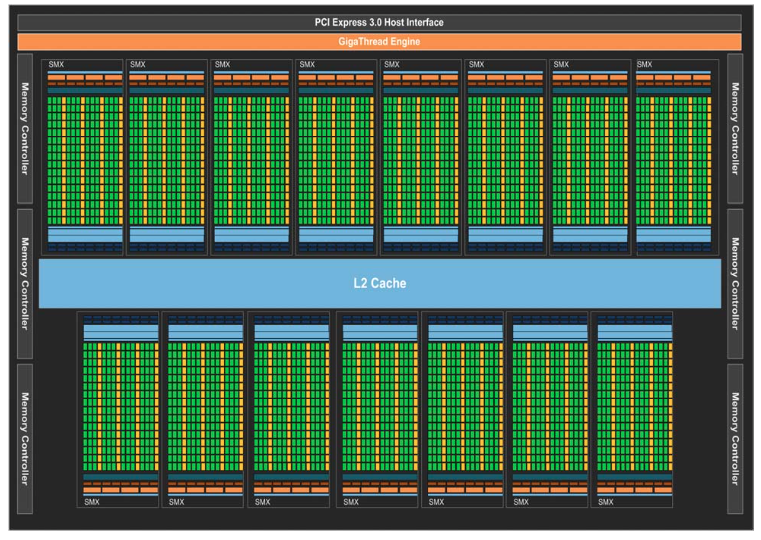
\includegraphics[width=0.5\textwidth]{figures/gpu_arch.png}
    \caption{Kepler GK110 architecture\cite{gpu_specs1}.}
    \label{GpuArch}
\end{figure}

\subsubsection{Mapping}
\par{The CUDA architecture is a scalar architecture. Therefore, there is no 
    performance benefit from using vector types and 
    instructions, a \emph{work item} is executed on a scalar processor and 
    \emph{work groups} are executed on multiprocessors(SMX)
    \cite{gpu_opencl_cuda,gpu_opencl_opt_slides}. A summary of the mapping of
    OpenCL to a GPU is shown in figure \ref{GpuModel}}

\par{Only one \emph{kernel} can execute in a device at one time. 
    \emph{Work groups} divide into groups of 32 threads called warps. 
    Warps always perform the same instruction and they are basic scheduling 
    units \cite{gpu_opencl_opt_slides}.}

\begin{figure}[!h]
    \centering
    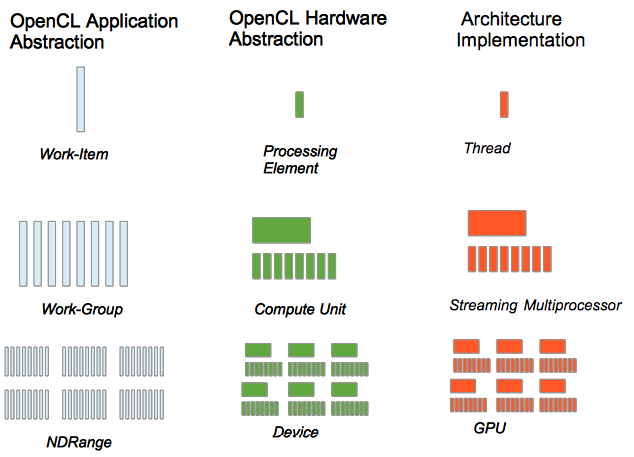
\includegraphics[width=0.5\textwidth]{figures/gpu_model.png}
    \caption{OpenCL mapping for GPU.}
    \label{GpuModel}
\end{figure}


\par{OpenCL \emph{private memory} is implemented as registers in the GPU, \emph{local memory} is implemented as shared memory 
    in the GPU\cite{gpu_opencl_opt_slides}.}

\par{If branching happens within a warp, different execution paths must be serialized, increasing the total number of 
    instructions although there is no penalty if different warps diverge\cite{gpu_opencl_opt_slides}.}

\begin{figure}[!h]
    \centering
    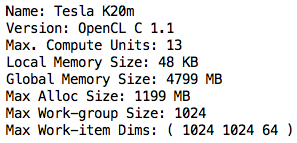
\includegraphics[width=0.35\textwidth]{figures/gpu_device_info.png}
    \caption{GPU device information.}
    \label{GpuDeviceInfo}
\end{figure}

\par{Figure \ref{GpuDeviceInfo} shows the information of the device gathered by OpenCL function calls, first thing to notice is 
    the version of OpenCL released by Nvidia(1.1) older than the one released by intel, OpenCL 1.2 has been released almost 4 years
    ago and still it is not available for Nvidia GPUs. Figure \ref{GpuDeviceInfo} also shows the number of \emph{compute units}(13),
    which is the number of Streaming Multiprocessors available in the device and approximatelly 5GB of Ram memory
    (\emph{global memory}).}




